% !TeX root = ../../main.tex
\newpage
\section{Wyniki zmodyfikowanej sieci}
\label{sec:wyniki_zmodyfikowanej}

\begin{table}[!h]
	\centering
	\caption{Wyniki na zbiorze \textit{low}}
	\vspace{6pt}
	{\footnotesize
		\begin{tabular}{|c|c|c|c|c|}
			\hline \textbackslash & True Positive & False Positive & False Negative & True Negative \\
      \hline Średnia & 277207.88 (48.34\%) & 401.75 (0.07\%) & 15599.04 (2.72\%) & 280231.33 (48.87\%) \\
      \hline Minimum & 151642 (26.44\%) & 0 (0.0\%) & 6631 (1.16\%) & 63840 (11.13\%) \\
      \hline Maksimum & 469357 (81.85\%) & 5575 (0.97\%) & 40243 (7.02\%) & 414522 (72.29\%) \\
      \hline Mediana & 271734.0 (47.39\%) & 131.0 (0.02\%) & 13172.0 (2.3\%) & 285509.0 (49.79\%) \\
      \hline
		\end{tabular}
	}
	\vspace{0pt}
\end{table}

\vspace{1cm}

\begin{figure}[!htb]
  \minipage{0.45\textwidth}
    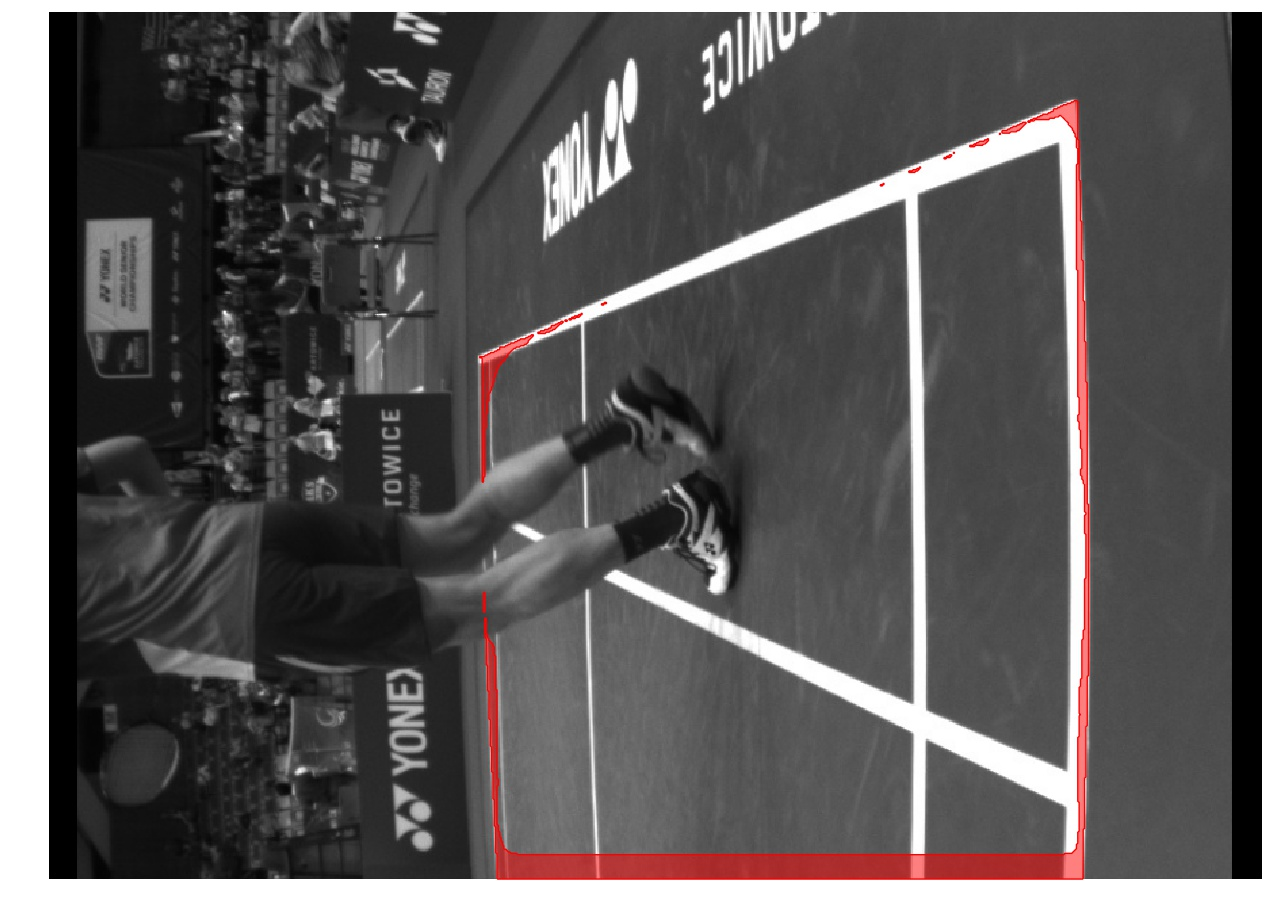
\includegraphics[width=\linewidth]{56_fn_1564911595553287247.jpg}
    \caption{Poglądowy obraz z zaznaczonym obszarem FN}
  \endminipage\hfill
  \minipage{0.45\textwidth}
    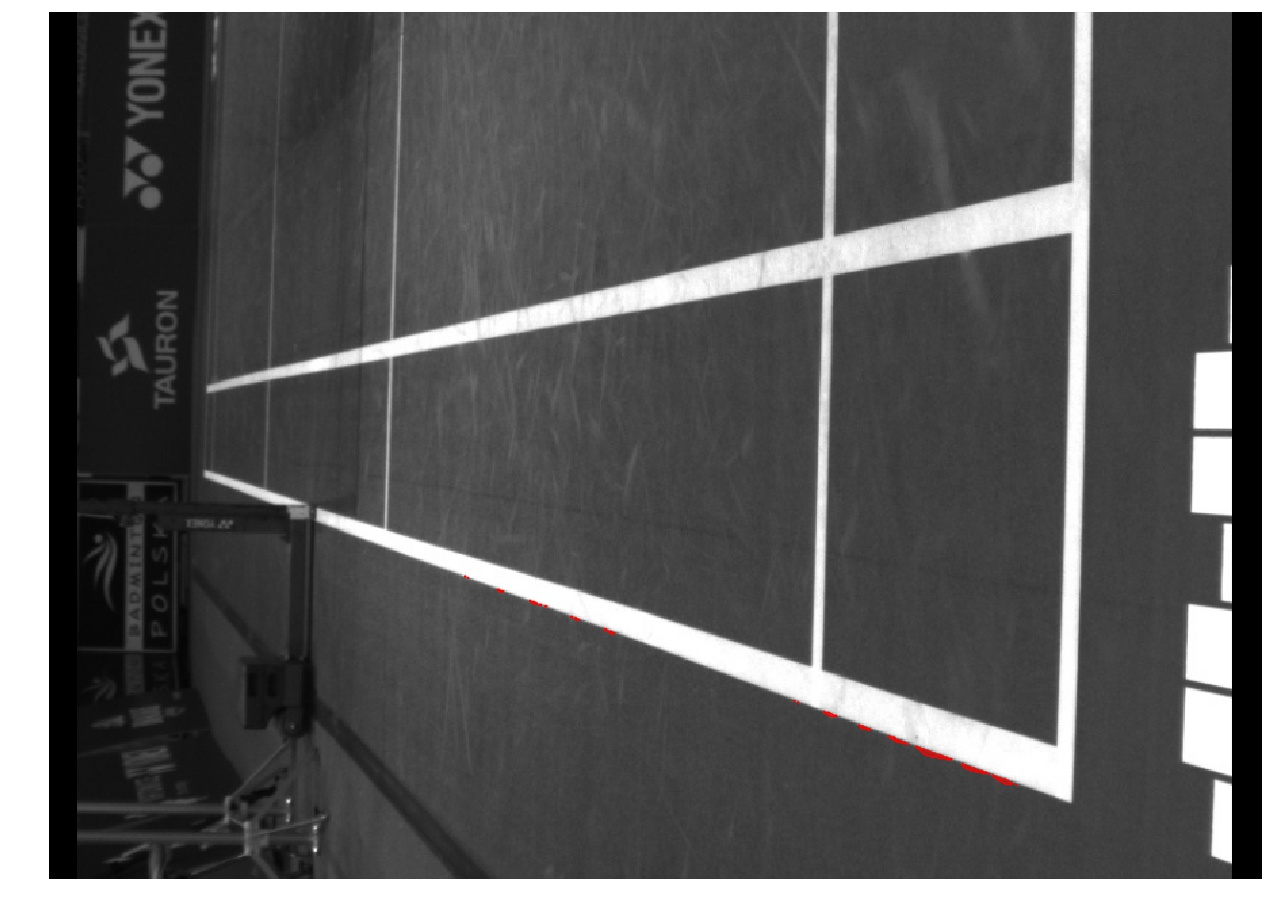
\includegraphics[width=\linewidth]{56_fp_1564953159296706208_5.jpg}
    \caption{Poglądowy obraz z zaznaczonym obszarem FP}
  \endminipage\hfill
\end{figure}

\vspace{1cm}

\begin{table}[!h]
	\centering
	\caption{Złożone wyniki \textit{low}}
	\vspace{6pt}
	{\footnotesize
		\begin{tabular}{|c|c|c|c|c|}
			\hline \textbackslash & Accuracy & Sensitivity & Specificity & Precision \\
      \hline Średnia & 0.97 & 0.95 & 1.0 & 1.0 \\
      \hline Minimum & 0.93 & 0.92 & 0.98 & 0.98 \\
      \hline Maksimum & 0.99 & 0.96 & 1.0 & 1.0 \\
      \hline Mediana & 0.97 & 0.95 & 1.0 & 1.0 \\
      \hline
		\end{tabular}
	}
	\vspace{0pt}
\end{table}

%loss - 0.01689
%val_loss = 0.03299
%val_mask_rcnn_loss = 0.01562

\missingfigure{
  Tu będzie wykres rezultatów \textbf{zmodyfikowanej} sieci Mask R-CNN \newline
  Na zbiorze \textbf{bez sztucznych danych}
}

\missingfigure{Tu będzie screenshot ilustrujący \textbf{rozwiązany} problem ``Falbanek''}

